\documentclass[../differential_forms.tex]{subfiles}
\begin{document}
\section{Aula 01 - 13 de Agosto, 2025}
\subsection{Motivações}
\begin{itemize}
	\item Relembrando Cálculo.
\end{itemize}
\subsection{Relembrando Cálculo}
O intuito dessa aula é fazer uma breve revisão, em partes informal, de alguns conceitos vistos ao longo do curso de matemática antes de adentrar no assunto de formas.
\begin{def*}
	Um \textbf{campo vetorial em }\(\mathbb{R}^{n}\) é uma função
	\begin{align*}
		\vec{F}:\Omega & \substack{\mathrm{ab}                                                                                                                                  \\ \subseteq }\mathbb{R}^{n} \rightarrow \mathbb{R}^{n} \\
		               & (x_1, \dotsc , x_{n})\longmapsto \vec{F}(x_1, \dotsc , x_{n}) \coloneqq (F_1(x_1, \dotsc , x_{n}), \dotsc , F_{n}(x_1, \dotsc , x_{n})). \quad \square
	\end{align*}
\end{def*}
\begin{figure}[H]
	\begin{center}
		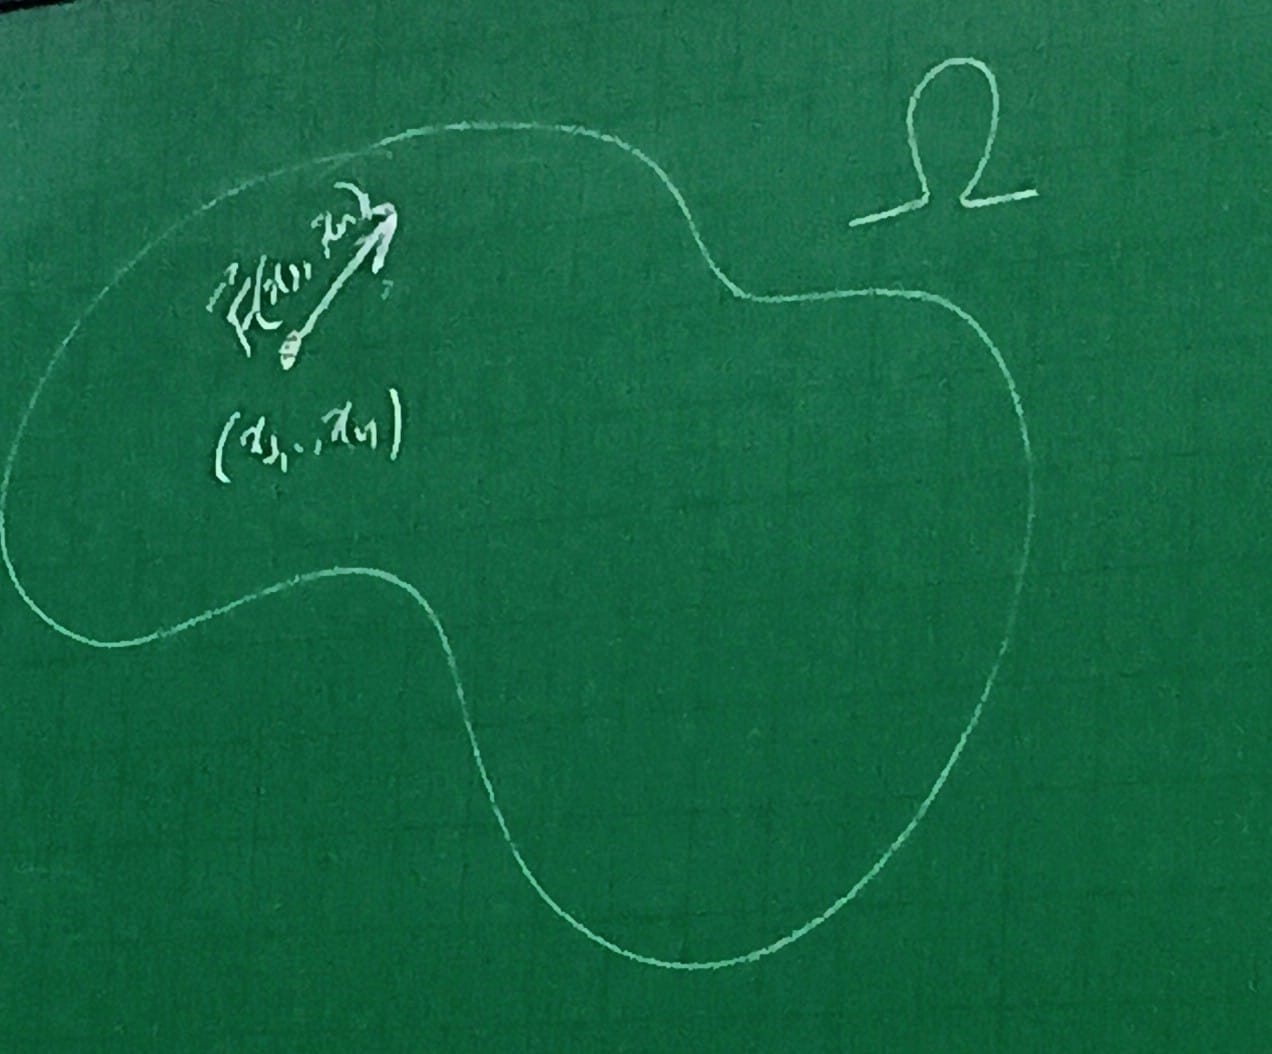
\includegraphics[height=0.5\textheight, width=0.5\textwidth, keepaspectratio]{./Images/vector_field_01.png}
	\end{center}
	\caption{a imagem de um campo de vetores normalmente é representada com setas -- vetores!}
\end{figure}

Veremos bastante a aparição de superfícies, sendo
\begin{def*}
	Uma \textbf{superfície} S pode ser vista como a imagem uma função \textit{regular} de classe \(\mathcal{C}^{1}\) em suas coordenadas, da forma
	\begin{align*}
		\sigma :  K\subseteq U & \substack{\mathrm{ab}                                                                                   \\ \subseteq }\mathbb{R}^{2}\rightarrow \mathbb{R}^{3} \\
		                       & (\mu , \sigma )\longmapsto (\sigma_1(\mu , \sigma ), \sigma_2(\mu , \sigma ), \sigma_3(\mu , \sigma )),
	\end{align*}
	com cada \(\sigma_{i}\) de classe \(\mathcal{C}^{1}.\; \square\)
\end{def*}
\begin{figure}[H]
	\begin{center}
		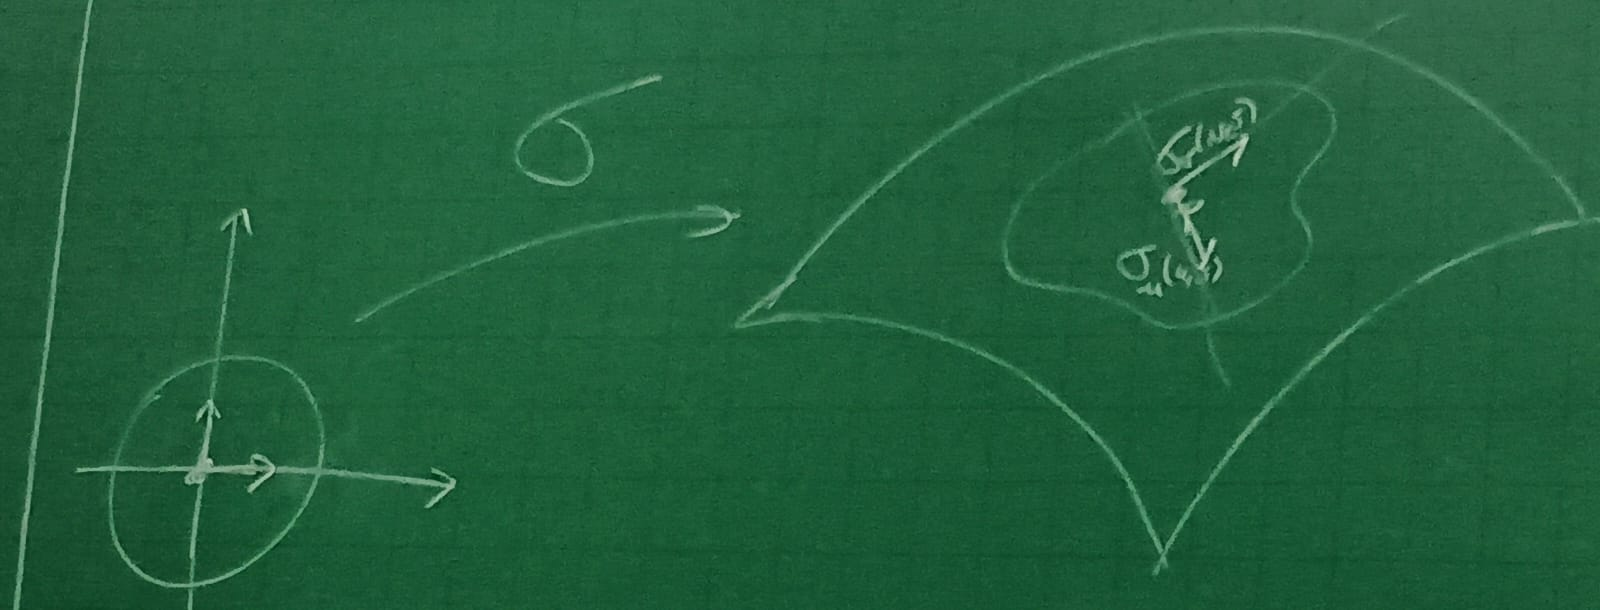
\includegraphics[height=0.5\textheight, width=0.5\textwidth, keepaspectratio]{./Images/surface_01.png}
	\end{center}
	\caption{representação típico de uma superfície, buscando associar uma \textit{malha} de \(\mathbb{R}^{2}\) com outra em \(\mathbb{R}^{3}\).}
\end{figure}

Tendo a noção de superfícies, também podemos definir o plano de vetores tangentes a uma superfície, o (convenientemente) chamado \textit{espaço tangente}, que possuí diferentes formas de definir, com uma mais útil a cada área da matemática, mas que buscam todas capturar a mesma ideia: alguma forma de generalização de derivadas, de velocidade ou de reta tangente, mas para outras dimensões. Melhor ainda, tendo em mente a visão da reta tangente como a melhor aproximação linear que se tem de uma curva, o plano tangente a uma superfície seria a melhor aproximação linear que se tem de um plano, e isso é o próprio \(\mathbb{R}^{2}\); isto vale para abertos de \(\mathbb{R}^{n}\) em geral: dado um aberto U de \(\mathbb{R}^{n}\), o plano tangente a pontos deste aberto é o próprio \(\mathbb{R}^{n}.\)

Vamos ver alguns exemplos de contas que podemos fazer nestes contextos:
\begin{example}
	Para calcular a integral
	\[
		\int_{\gamma }^{}\vec{F} \mathrm{dr},
	\]
	sendo
	\[
		\vec{F}(x, y) = x \vec{i} + y \vec{j} \quad\&\quad \gamma (t) = (t, t^{2}),\; t\in [-1, 1],
	\]
	fazemos
	\[
		\int_{\gamma }^{} \vec{F} \mathrm{d\gamma } = \int_{[a, b]}^{}\vec{F}\circ \gamma (t) \cdot \gamma'(t) \mathrm{dt} = \int_{-1}^{1}\vec{F}(\gamma (t))\cdot \gamma '(t) \mathrm{dt},
	\]
	que o significado deste produto escalar feito corretamente é de uma \textit{projeção!} Especificamente, uma projeção originada dos funcionais lineares\footnote{E já é um exemplo de uma 1-forma, como veremos mais pra frente.}. Neste caso,
	\[
		\vec{F}(\gamma (t)) = \vec{F}(t, t^{2}) = \underbrace{t \vec{i} + t^{2} \vec{j}}_{\mathclap{\substack{\text{está no } \\ \text{espaço tangente}}}} \quad\&\quad \underbrace{\gamma '(t) = (1, 2t)}_{\mathclap{\text{está no espaço tangente}}},
	\]
	e, pela forma que é normalmente definida, teremos
	\begin{align*}
		\int_{\gamma }^{}\vec{F} \mathrm{d\gamma } = \int_{-1}^{1} \vec{F}(\gamma (t))\cdot \gamma '(t) \mathrm{dt} & = \int_{-1}^{1}(t \vec{i} + t^{2}\vec{j})\cdot (1, 2t) \mathrm{dt} \\
		                                                                                                            & = \int_{-1}^{1} (t+2t^{3}) \mathrm{dt}  = 0.
	\end{align*}

\end{example}
\begin{tcolorbox}[
		skin=enhanced,
		title=Observação,
		fonttitle=\bfseries,
		colframe=black,
		colbacktitle=cyan!75!white,
		colback=cyan!15,
		colbacklower=black,
		coltitle=black,
		drop fuzzy shadow,
		%drop large lifted shadow
	]
	Toda a parte da notação do exemplo acima passará a ser reinterpretado após a introdução de um dos principais objetos de estudo daqui -- as \textbf{\textit{formas}}.
\end{tcolorbox}

\subsection{Operadores Diferenciais}
Ao longo da matemática, também vimos alguns operadores diferenciais que valem a pena ser revisados; dentre eles, temos
\begin{itemize}
	\item \textbf{\underline{Gradiente}:} o gradiente de uma função escalar \(f:\mathbb{R}^{n}\rightarrow \mathbb{R}\) é
	      \[
		      \nabla f = \biggl(\frac{\partial^{}f}{\partial x_1^{}}, \frac{\partial^{}f}{\partial x_{n}^{}}\biggr),
	      \]
	      que servem como coeficientes do funcional linear.
	\item \textbf{\underline{Divergente}:} para um campo de vetores \(\vec{F}\), o seu divergente é dado por
	      \[
		      \nabla \cdot \vec{F} = \sum\limits_{i=1}^{n}\frac{\partial^{}F_{i}}{\partial x_{i}^{}};
	      \]
	\item \textbf{\underline{Rotacional}:} Novamente para um campo de vetores \(\vec{F}\), sua rotacional é dada por
	      \[
		      \mathrm{rot}(\vec{F}) = \biggl(\frac{\partial^{}F_3}{\partial y^{}} - \frac{\partial^{}F_2}{\partial x^{}}, \frac{\partial^{}F_1}{\partial x^{}} - \frac{\partial^{}F_3}{\partial x^{}}, \frac{\partial^{}F_2}{\partial x^{}} - \frac{\partial^{}F_1}{\partial y^{}}\biggr).
	      \]
\end{itemize}
Com estes operadores, outro resultado torna-se particularmente importante de ser relembrado:
\hypertarget{green_theorem_calc}{
	\begin{theorem*}[Teorema de Green]
		Seja \(K\) um compacto com interior não vazio em \(\mathbb{R}^{2}\), cuja fronteira é a imagem de uma curva \(\gamma : [a, b]\rightarrow \mathbb{R}^{2}\) fechada, simples, \(\mathcal{C}^{1}\) por partes e orientada no sentido anti-horário. Além disso, seja \(F(x, y) = P(x, y)\vec{i} + Q(x, y)\vec{j}\), onde P e Q são de classe \(\mathcal{C}^{1}\) em um aberto contendo K. Nestas condições,
		\[
			\oint_{\gamma }Pdx = \iint_{K}\biggl[\frac{\partial^{}Q}{\partial x^{}} - \frac{\partial^{}P}{\partial y^{}}\biggr]\mathrm{d}x \mathrm{d}y.
		\]
	\end{theorem*}
}
\end{document}
